\section{Problem Set \#1}
\pagenumbering{arabic}

\begin{exercise}
    Let \(X_{1}, \cdots, X_{n}\) be a random sample from the a.c. distribution
    \[
    f(x \mid \theta)=\theta x^{\theta-1} 1_{\{0 \leqslant x \leqslant 1\}}, \quad 0<\theta<\infty .
    \]
    Find the method of moments estimator of \(\theta\).
\end{exercise}

\begin{solution}
    For the sample \(\{X_i\}_{i=1}^n\), 
    \[
        \begin{aligned}
            \bar{X}=\mu_1=E(X_i)&=\int_0^1xf(x)\der x=\int_0^1\theta x^\theta\der x\\
            &=\frac{\theta}{\theta+1}x^{\theta+1}\big|_0^1=\frac{\theta}{\theta+1}. 
        \end{aligned}
    \]
    So, the method of moments estimator for $\theta$ is 
    \[
        \hat{\mu}_1=\frac{1}{n}\sum_{i=1}^nX_i=\frac{\theta}{\theta+1}
    \]
    \[
        \hat{\theta}=\frac{\hat{\mu}_1}{1-\hat{\mu}_1}. 
    \]
\end{solution}

\begin{exercise}
    Let \(X_{1}, \cdots, X_{n} \stackrel{\text { i.i.d. }}{\sim} \operatorname{Geo}(p), 0<p<1\), i.e.,
    \[
    \mathbb{P}\left(X_{1}=k \mid p\right)=(1-p)^{k-1} p, \quad k \in \mathbb{N} .
    \]
    What is the method of moments estimator of \(p\) ?
\end{exercise}

\begin{solution}
    For the sample \(\{X_i\}_{i=1}^n\), 
    \[
        \begin{aligned}
            \bar{X}=\mu_1=E(X_i)&=\sum_{k=0}^\infty k\cdot (1-p)^{k-1}p=\frac{1-p}{p}
        \end{aligned}
    \]
    So, the method of moments estimator of $p$ is 
    \[
        \hat{\mu}_1=\frac{1}{n}\sum_{i=1}^nX_i=\frac{1-p}{p}
    \]
    \[
        \hat{p}=\frac{1}{\hat{\mu}_1+1}. 
    \]
\end{solution}
    
\begin{exercise}
    Assume \(X \sim B(n, p)\), where both \(n \in \mathbb{N}\) and \(p \in(0,1)\) are unknown. Given a random sample of \(N\) observations of \(X\), compute the method of moments estimator of \(n\) and \(p\).
\end{exercise}

\begin{solution}
    For the sample \(\{X_i\}_{i=1}^N\), 
    \[
        \bar{X}=\mu_1=E(X_i)=\sum_{k=0}^nk\cdot \binom{n}{k}p^k(1-p)^{n-k}=np, 
    \]
    \[
        Var(X_i)=E(X_i^2)-(E(X_i))^2=\mu_2-\mu^2=np(1-p), 
    \]
    Now, solve these two equations: 
    \[
        \left\{\begin{array}{l}
            \hat{\mu}_1=np\\
            \hat{\mu}_2-\hat{\mu}_1^2=np(1-p)
        \end{array}\right.
    \]
    We can get that
    \[
        \hat{p}=1-\frac{\hat{\mu}_2-\hat{\mu}_1^2}{\hat{\mu}_1},\qquad\hat{n}=\frac{\hat{\mu}_1^2}{\hat{\mu}_1-\hat{\mu}_2+\hat{\mu}_1^2}. 
    \]
\end{solution}

\begin{exercise}
    Let \(X_{1}, \cdots, X_{n}\) be a random sample from the density
    \[
    f(x \mid \theta)=\theta x^{-2}, \quad 0<\theta \leqslant x<\infty .
    \]
    What can you say about the existence of the method of moments estimator of \(\theta\) ?
\end{exercise}

\begin{solution}
    \[
        E(X_i)=\int_{\theta}^\infty x\cdot \theta x^{-2}\der x=\theta \ln x \big|_\theta^\infty=\theta(\ln\infty-\ln\theta)=\infty, 
    \]
    So, the method of moments estimator for \(\theta\) does not exist. 
\end{solution}

\begin{exercise}
    Show that each of the following is an exponential family and describe the natural parameter space \(\mathcal{E}\) of the associated canonical exponential family.
    \begin{enumerate}[(a)]
        \item \(\{\Gamma(\alpha, \lambda)\}_{\alpha, \lambda>0}\), i.e.,
        \[
        f(x \mid \alpha, \lambda)=\frac{\lambda^{\alpha}}{\Gamma(\alpha)} x^{\alpha-1} e^{-\lambda x} 1_{\{x>0\}} ;
        \]
        \item \(\{\operatorname{Beta}(a, b)\}_{a, b>0}\), i.e.,
        \[
        f(x \mid a, b)=\frac{\Gamma(a+b)}{\Gamma(a) \Gamma(b)} x^{a-1}(1-x)^{b-1} 1_{\{0<x<1\}} ;
        \]
        \item \(\{\operatorname{Poi}(\lambda)\}_{\lambda>0}\);
        \item \(\{\operatorname{NegBin}(r, p)\}_{0 \leqslant p \leqslant 1}(r\) being known), i.e.,
        \[
        f(x \mid p)=\left(\begin{array}{c}
        r+x-1 \\
        x
        \end{array}\right) p^{r}(1-p)^{x}, \quad x \in \mathbb{N} \cup\{0\} .
        \]
    \end{enumerate}
\end{exercise}

\begin{solution}
    \begin{enumerate}[(a)]
        \item
        \[
            \begin{aligned}
                f(x|\alpha, \lambda)&=1_{\{x>0\}}\exp(\alpha\ln(\lambda)-\ln(\Gamma(\alpha))+(\alpha-1)\ln(x)-\lambda x)\\
                &=1_{\{x>0\}}\exp((\alpha-1)\ln(x)-\lambda x+\alpha\ln(\lambda)-\ln(\Gamma(\alpha))), 
            \end{aligned}
        \]
        So, the nature parameter is $(\eta_1,\eta_2)=(\alpha-1, -\lambda)$. And the parameter space \(\mathcal{E}\) is \((-1,\infty)\times(-\infty,0)\). 
        \item
        \[
            \begin{aligned}
                f(x|a,b)=1_{\{0<x<1\}}&\exp((a-1)\ln(x)+(b-1)\ln(1-x)\\&+\ln(\Gamma(a+b))-\ln(\Gamma(a))-\ln(\Gamma(b))), 
            \end{aligned}
        \] 
        So, the nature parameter is $(\eta_1,\eta_2)=(a-1, b-1)$. And the parameter space \(\mathcal{E}\) is \((-1,\infty)\times(-1,\infty)\). 
        \item When \(k\in\mathbb{N}\), 
        \[
            f(x)=P(X=k)=\frac{e^{-\lambda}\lambda^k}{k!}
        \]
        \[
            \begin{aligned}
                P(X=k)=&1/k!\cdot\exp(-\lambda+k\ln(\lambda)), 
            \end{aligned}
        \]
        So, the nature parameter is $(\eta)=(\ln(\lambda))$. And the parameter space \(\mathcal{E}\) is \((-\infty,\infty)\). 
        \item When \(x\in\mathbb{N}\), 
        \[
            \begin{aligned}
                f(x|p)&=\binom{r+x-1}{x}\exp\left(r\ln(p)+x\ln(1-p)\right), 
            \end{aligned}
        \]
        So, the nature parameter is $(\eta)=(\ln(1-p))$. And the parameter space \(\mathcal{E}\) is \((-\infty,0]\). 
    \end{enumerate}
\end{solution}

\begin{exercise}
    In \(n\) independent trials with \(k+1\) possible outcomes, let the probability of the \(i\)-th outcome be \(p_{i}\) in each trial. If \(X_{i}\) denotes the number of trials resulting in outcome \(i, i=0,1, \ldots, k\), then the joint distribution of \(X\) is the multinomial distribution, i.e., 
    \[
        f(\mathbf{x} \mid \mathbf{p}):=\mathbb{P}\left(X_{0}=x_{0}, X_{1}=x_{1}, \ldots, X_{k}=x_{k} \mid \mathbf{p}\right)=\frac{n !}{x_{0} ! x_{1} ! \ldots x_{k} !} p_{0}^{x_{0}} p_{1}^{x_{1}} \ldots p_{k}^{x_{k}}. 
    \]
    \begin{enumerate}[(a)]
        \item Verify that \(\{f(\mathbf{x} \mid \mathbf{p})\}_{\mathbf{p} \in \Pi_{k}}\) is an exponential family, where \(\Pi_{k}\) is the \(k\)-dimensional simplex in \(\mathbb{R}^{k+1}\). Determine \(\mathcal{E}\). 
        \item Using results for canonical exponential families, show that
        \[
            \mathbb{E} X_{i}=n p_{i}, \quad \operatorname{Cov}\left(X_{j}, X_{i}\right)=\left\{\begin{array}{cc}
            n p_{j}\left(1-p_{j}\right), & k=j \\
            -n p_{j} p_{k}, & k \neq j
        \end{array}\right.
        \]
    \end{enumerate}
\end{exercise}

\begin{solution}
    \begin{enumerate}[(a)]
        \item We know for every $p_i$, \(0\leqslant p_i\leqslant 1\). 
        \[
            f(x|\mathbf{p})=\frac{n !}{x_{0} ! x_{1} ! \ldots x_{k} !} \exp\left(x_0\ln (p_0)+\cdots+x_k\ln (p_k)\right). 
        \]
        So, the nature parameter is $(\eta_0,\cdots,\eta_k)=(\ln(p_0),\cdots,\ln(p_k))$. And the parameter space \(\mathcal{E}\) is \((-\infty,0]\times\cdots\times(-\infty,0]\). 
        \item Noting this $p_{k}=1-\sum_{i=0}^{k-1}p_i$, we can parameterize the distribution as:
        \[
            \begin{aligned}
                f(x|\mathbf{p})&=\frac{n!}{x_0!x_1!\cdots x_k!}\exp\left\{\sum_{i=0}^{k-1}\ln(p_i)x_i+\left(n-\sum_{i=0}^{k-1}x_i\right)\ln\left(1-\sum_{i=0}^{k-1}p_i\right)\right\}\\
                &=\frac{n!}{x_0!x_1!\cdots x_k!}\exp\left\{\sum_{i=0}^{k-1}\ln\left(\frac{p_i}{1-\sum_{i=0}^{k-1}p_i}\right)x_i+n\ln\left(1-\sum_{i=0}^{k-1}p_i\right)\right\}. 
            \end{aligned}
        \]
        Let $\eta_i=\ln\left(\frac{p_i}{1-\sum_{i=0}^{k-1}p_i}\right)$, then we know $p_i=\frac{e^{\eta_i}}{\sum_{i=0}^ke^{\eta_i}}$. So, 
        \[
            \begin{aligned}
                A(\eta)=n\ln\left(\sum_{i=0}^ke^{\eta_i}\right). 
            \end{aligned}
        \]
        So, 
        \[
            \mathbb{E}X_i=A_{\eta_i}'(\eta)=n\frac{e^{\eta_i}}{\sum_{i=0}^ke^{\eta_i}}=np_i. 
        \]
        When $i=j$, 
        \[
            \text{Cov}(X_j,X_i)=A_{\eta_i}''(\eta)=n\frac{e^{\eta_i}(\sum_{i=0}^k)e^{\eta_i}-e^{\eta_i}e^{\eta_i}}{\sum_{i=0}^ke^{\eta_i}}=np_i(1-p_i). 
        \]
        When $i\not=j$, 
        \[
            \text{Cov}(X_j,X_i)=\frac{A(\eta)}{\partial\eta_i\,\partial\eta_j}=ne^{\eta_i}\frac{-e^{\eta_j}}{(\sum_{i=0}^ke^{\eta_i})^2}=-np_ip_j. 
        \]
    \end{enumerate}
\end{solution}

\begin{exercise}
    The Inverse Gaussian density, \(I G(\mu, \lambda)\), is given by
    \[
        f(x \mid \mu, \lambda)=\left(\frac{\lambda}{2 \pi}\right)^{1 / 2} x^{-3 / 2} \exp \left\{\frac{-\lambda(x-\mu)^{2}}{2 \mu^{2} x}\right\}, \quad x>0, \quad \mu>0, \quad \lambda>0. 
    \]
    \begin{enumerate}[(a)]
        \item Show that this is an exponential family generated by \(T(X)=-\frac{1}{2}\left(X, X^{-1}\right)^{T}\) and \(h(x)=\) \((2 \pi)^{-1 / 2} x^{-3 / 2}\). 
        \item Show that the canonical parameters \(\eta_{1}, \eta_{2}\) are given by \(\eta_{1}=\mu^{-2} \lambda, \eta_{2}=\lambda\), and that \(A\left(\eta_{1}, \eta_{2}\right)=-\left(\frac{1}{2} \log \left(\eta_{2}\right)+\sqrt{\eta_{1} \eta_{2}}\right), \mathcal{E}=[0, \infty) \times(0, \infty)\). 
        \item Find the moment generating function of \(T\) and show that \(\mathbb{E}(X)=\mu, \operatorname{Var}(X)=\mu^{3} \lambda^{-1}\), \(\mathbb{E}\left(X^{-1}\right)=\mu^{-1}+\lambda^{-1}, \operatorname{Var}\left(X^{-1}\right)=(\lambda \mu)^{-1}+2 \lambda^{-2} .\)
    \end{enumerate}
\end{exercise}

\begin{solution}
    \begin{enumerate}[(a)]
        \item \[
            \begin{aligned}
                f(x|\mu,\lambda)&=(2 \pi)^{-1 / 2} x^{-3 / 2}\exp\left\{-\lambda(x^2-2\mu x+\mu^2)\cdot(2\mu^2x)^{-1}+\frac{1}{2}\ln(\lambda)\right\}\\
                &=(2 \pi)^{-1 / 2} x^{-3 / 2}\exp\left\{\frac{-\lambda}{2\mu^2}x + \frac{\lambda}{\mu}-\frac{\lambda}{2}x^{-1}+\frac{1}{2}\ln(\lambda)\right\}
            \end{aligned}
        \]
        So, $T(X)=-\frac{1}{2}(X,X^{-1})$, \(h(x)=\) \((2 \pi)^{-1 / 2} x^{-3 / 2}\). 
        \item $B((\lambda, \mu))=-(1/2\ln(\lambda)+\lambda/\mu)$, and $\eta=(\eta_1,\eta_2)=(\lambda/\mu^2, \lambda)$. So, 
        \[
            A(\eta)=-(1/2\ln(\eta_2)+(\eta_1\eta_2)^{1/2}). 
        \]
        \item The moment-generating function of $T(X)$ is
        \[
            M(s)=\exp\left(A(s+\eta)-A(\eta)\right). 
        \]
        And
        \[
            \mathbb{E}(-1/2X)=A_{\eta_1}'(\eta)=-(1/2(\eta_1\eta_2)^{-1/2}\eta_2)=-1/2\mu,\quad \mathbb{E}X=\mu. 
        \]
        \[
            \text{Var}(-1/2X)=A_{\eta_1}''(\eta)=1/4(\eta_1\eta_2)^{-3/2}\eta_2^2=1/4\mu^3\lambda^{-1},\quad \text{Var}(X)=\mu^3\lambda^{-1}. 
        \]
        \[
            \mathbb{E}(-1/2X^{-1})=A_{\eta_2}'(\eta)=-(1/2\eta_2^{-1}+1/2(\eta_1\eta_2)^{-1/2}\eta_1)=-1/2(\mu^{-1}+\lambda^{-1}), 
        \]
        \[
            \mathbb{E}(X^{-1})=\mu^{-1}+\lambda^{-1}. 
        \]
        \[
            \text{Var}(-1/2X^{-1})=A_{\eta_2}''(\eta)=1/2\eta_2^{-2}+1/4(\eta_1\eta_2)^{-3/2}\eta_1^2=1/2\lambda^{-2}+1/4(\lambda^{-1}\mu^{-1}),
        \]
        \[
            \text{Var}(X^{-1})=2\lambda^{-2}+(\lambda\mu)^{-1}. 
        \]
    \end{enumerate}
\end{solution}

\begin{exercise}
    For each of the following families: \((i)\) verify that it is an exponential family; \((i i)\) describe the curve in which the parameter vector \(\theta\) lies (with respect to the natural parametrization). 
    \begin{enumerate}[(a)]
        \item \(\left\{\mathcal{N}\left(\theta, a \theta^{2}\right)\right\}_{\theta \in \mathbb{R}}, a\) is known;
        \item \(\{\Gamma(\alpha, \alpha)\}_{\alpha>0} ;\)
        \item \(\{f(x \mid \theta)\}_{\theta \in \mathbb{R}}\), where \(f(x \mid \theta)=C \exp \left\{-(x-\theta)^{4}\right\}, x \in \mathbb{R}\), and \(C\) is a normalizing constant.
    \end{enumerate}
\end{exercise}

\begin{solution}
    \begin{enumerate}[(a)]
        \item 
        \begin{enumerate}[(a)]
            \item[(i)] The density function of normal distribution can be write as: 
            \[
                \begin{aligned}
                    f(x|\theta)&={\frac {1}{{\sqrt {2\pi a}\theta}}}\;\exp\left(-{\frac {\left(x-\theta \right)^{2}}{2a\theta^2}}\right)\\
                    &=e^{-\frac{1}{2a}}\exp\left(-\frac{1}{2a\theta^2}x^2+\frac{1}{a\theta}x-\ln(\sqrt{2\pi a}\theta)\right). 
                \end{aligned}
            \]
            $h(x)=e^{-\frac{1}{2a}}1_{-\infty<x<\infty}$, $\eta=\left(-\frac{1}{2a\theta^2}, \frac{1}{a\theta}\right)$, $T(X)=(x^2, x)$. 
            \item[(ii)]
            Let $u=-\frac{1}{2a\theta^2}$, $v=\frac{1}{a\theta}$, then
            \[
                u=-\frac{a}{2}v^2. 
            \]
            It is a parabola. 
        \end{enumerate}
        \item 
        \begin{enumerate}[(a)]
            \item[(i)]
            \[
                \begin{aligned}
                    f(x \mid \alpha, \alpha)&=\frac{\alpha^{\alpha}}{\Gamma(\alpha)} x^{\alpha-1} e^{-\alpha x} 1_{\{x>0\}}\\
                    &=\exp\left(-\alpha x+(\alpha-1)\ln(x)+\alpha\ln(\alpha)-\ln(\Gamma(\alpha))\right)1_{\{x>0\}}
                \end{aligned}
            \]
            $h(x)=1_{\{x>0\}}$, $T(X)=(x, \ln(x))$, $\eta=(-\alpha,\alpha-1)$. 
            \item[(ii)] 
            Let $u=-\alpha$, $v=\alpha-1$, then
            \[
                v=-u-1,\quad u<0.  
            \]
            It is a line. 
        \end{enumerate}
        \item
        \begin{enumerate}[(a)]
            \item[(i)]
            \[
                \begin{aligned}
                    f(x|\theta)&=C\exp(-(x-\theta)^4)\\
                    &=C\exp\left(-x^4+4\theta x^3-6\theta^2x^2+4\theta^3x-\theta^4\right)
                \end{aligned}
            \]
            $h(x)=C\exp(-x^4)1_{\{-\infty<x<\infty\}}$, $T(X)=(4x^3, -6x^2, 4x)$, $\eta=(\theta, \theta^2, \theta^3)$. 
            \item[(ii)] It is a spiral. In Mathematica, we can get the plot of the curve like this: 
\begin{minted}[breaklines]{mathematica}
ParametricPlot3D[{t, t^2, t^3}, {t, 0, 1}, {ViewPoint -> {1.3, -2.4, 2.}}]
\end{minted}            
            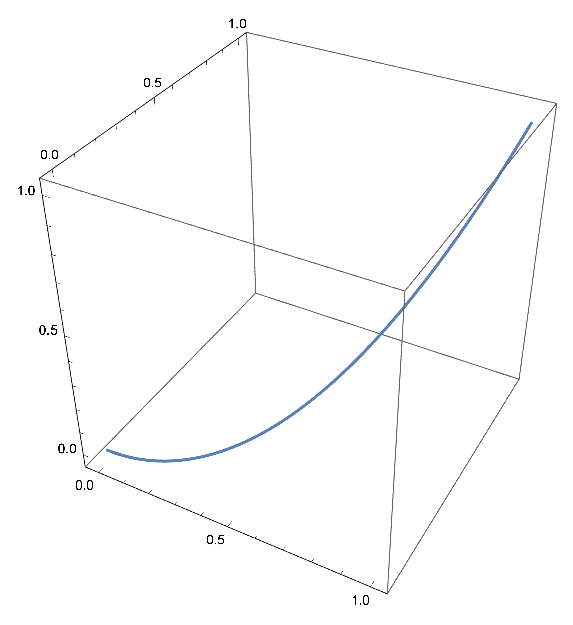
\includegraphics{1.8.c.eps}
        \end{enumerate}
    \end{enumerate}
\end{solution}

\begin{exercise}
    (In this problem, we generalize the proposition shown in class) 
    
    Let \(\{f(\mathbf{x} \mid \theta)\}_{\theta \in \Theta}\) be a \(k\) parameter exponential family generated by \((T, h)\). Show that the distribution for \(T(\mathbf{X})\) is also a \(k\)-parameter exponential family. Hint: let \(G_{*}(d \mathbf{x})=h(\mathbf{x}) G(d \mathbf{x})\) and define the induced probability measure
    \[
        \mathbb{P}_{T}(B):=\mathbb{P}(T(\mathbf{X}) \in B)=\int_{\mathbb{R}^{n}} 1_{B}(T(\mathbf{x})) \exp \{\langle W(\theta), T(\mathbf{x})\rangle-B(\theta)\} G_{*}(d \mathbf{x}), 
    \]
    for \(B \in \mathcal{B}\left(\mathbb{R}^{k}\right)\). Now recall the following fundamental result on changes of measure, established in the course Probability theory \(I\). 

    {\bfseries Theorem. (Meerschaert and Scheffler (2001), \(p .4)\)} If \(\mu(d x)\) is a measure on \(\mathcal{B}\left(\mathbb{R}^{d}\right)\) and if \(T: \mathbb{R}^{d} \rightarrow \mathbb{R}^{m}, f: \mathbb{R}^{m} \rightarrow \mathbb{R}^{n}\) are Borel measurable, then
    \[
        \int_{\mathbb{R}^{d}} f(T(\boldsymbol{x})) \mu(d \boldsymbol{x})=\int_{\mathbb{R}^{m}} f(\boldsymbol{y})(T \mu)(d \boldsymbol{y}),
    \]
    where we define the measure \((T \mu)(B)=\mu\left(T^{-1}(B)\right), B \in \mathcal{B}\left(\mathbb{R}^{m}\right)\). 
\end{exercise}

\begin{solution}
    Knowing that $f(x|\theta)$ is generated by $(T,h)$, i.e. 
    \[
        f(x|\eta)=h(x)\exp\left(\eta^TT(x)-A(\eta)\right), 
    \]
    \[
        A(\eta)=\log\int h(x)\exp\left(\sum\eta_iT_i(x)\right) \der x. 
    \]
    If we replace $x$ with $T(x)$, then 
    \[
        A'(\eta)=\log\int h(T^{-1}(t))\exp\left(\sum\eta_it_i\right)\left|\begin{matrix}
            \frac{\pder }{}
        \end{matrix}\right|
    \]
\end{solution}

\begin{exercise}
    Let \(\mathcal{E} \neq \emptyset\) be the natural parameter set of some canonical \(k\)-parameter exponential family, \(k \in \mathbb{N}\). Show that \(\operatorname{int}(\mathcal{E}) \neq \emptyset\) if and only if \(\mathcal{E}\) is not contained in any \((k-1)\)-dimensional hyperplane (suggestion: for the converse, set \(k=3\) to help visualize the problem and use the fact that \(\mathcal{E}\) is convex).
\end{exercise}

\begin{exercise}
    Let \(\{f(\cdot \mid \boldsymbol{\eta})\}_{\boldsymbol{\eta} \in \mathcal{E}}\) be an a.c. canonical \(k\)-parameter exponential family. Fix an event \(A\). 
    \begin{enumerate}[(a)]
        \item Prove that if \(\mathbb{P}_{\eta_{0}}(A)=0\) for some \(\eta_{0} \in \mathcal{E}\), then \(\mathbb{P}_{\eta}(A)=0\) for all \(\eta \in \mathcal{E}\). 
        \item Conclude that if \(\mathbb{P}_{\eta_{0}}(A)<1\) for some \(\eta_{0} \in \mathcal{E}\), then \(\mathbb{P}_{\eta}(A)<1\) for all \(\eta \in \mathcal{E}\).
    \end{enumerate}
\end{exercise}

\begin{exercise}
    Determine the natural parameter space \(\mathcal{E}\) of the a.c. one-parameter canonical exponential family \(\{f(. \mid \boldsymbol{\eta})\}_{\boldsymbol{\eta}}\) when \(T(x)=x\) and
    \begin{enumerate}[(a)]
        \item \(h(x)=e^{-|x|}\);
        \item \(h(x)=\frac{e^{-|x|}}{1+x^{2}}\).
    \end{enumerate}
    Conclude that the natural parameter space does not have to be an open set.
\end{exercise}


\begin{exercise}
    Consider a classical linear regression, i.e., assume we have a sample \(Y_{1}, \ldots, Y_{n}\) of independent random variables such that, for \(i=1, \ldots, n, Y_{i} \sim \mathcal{N}\left(\mu_{i}, \sigma^{2}\right), \mu_{i}=\beta_{1}+\beta_{2} z_{i}, \sigma^{2}>0, \beta_{1} \in \mathbb{R}\), \(\beta_{2} \in \mathbb{R}\). Show that this forms a canonical exponential family with natural parameter space \(\mathcal{E}=\mathbb{R} \times \mathbb{R} \times(-\infty, 0)\) up to a permutation of the latter three components.
\end{exercise}